\documentclass[10pt,a4paper]{article}
\usepackage[T1]{fontenc}
\usepackage[utf8]{inputenc}
\usepackage{mathptmx}
\usepackage[top=1.7cm,bottom=1.7cm,left=1.9cm,right=1.9cm]{geometry}
\usepackage{graphicx,booktabs,tabularx,array,xcolor,enumitem,microtype,caption,float}
\usepackage[colorlinks=true,urlcolor=blue!60!black,citecolor=black,linkcolor=black]{hyperref}

\setlength{\parindent}{0pt}
\setlength{\parskip}{0.45em}
\setlist{nosep,leftmargin=1.2em,topsep=0.2em}
\captionsetup{font=small,labelfont=bf,skip=3pt}
\newcolumntype{L}[1]{>{\raggedright\arraybackslash}p{#1}}
\newcolumntype{Y}{>{\raggedright\arraybackslash}X}
\renewcommand{\arraystretch}{1.15}

\makeatletter
\renewcommand\section{\@startsection{section}{1}{\z@}{0.9em}{0.35em}{\normalfont\large\bfseries}}
\makeatother

\begin{document}

{\LARGE\bfseries Using fewer tokens without losing answer quality\par}
\vspace{0.3em}
{\small Short technical exercise for the internship 2026-INT-298\\
Farah Belghith, ENSIT Tunis \textperiodcentered{} November 2026\\
Code, data and full answers: \url{https://github.com/Farah-Belghith2710/token-efficient-assistant}\par}
\vspace{0.4em}

\textbf{Why I chose this topic.}
Last summer, during my internship at TDS, I built a RAG chatbot~\cite{lewis} for an Industry~4.0 lab. It used Groq's free plan.
After testing it many times, I reached the daily limit of 100{,}000 tokens. This happened even though each question used only about 2\% of the model's context window.
I realised that the main issue was not the size of the context window. It was the number of tokens used across requests.
At the time, I only estimated token use by dividing the number of characters by four.
For this exercise, I wanted to measure it more accurately using the counts returned by the API, while also checking that the answers stayed correct.

\section*{A. Five ways to use fewer tokens}
Each assistant request contains several parts: instructions, chat history, passages found by search, the user's question and the answer.
I grouped the ideas below by the part they help reduce.

\begin{table}[h]
\centering\footnotesize
\begin{tabularx}{\textwidth}{L{2.4cm} Y Y Y}
\toprule
\textbf{Approach} & \textbf{How it works} & \textbf{Why it helps} & \textbf{What can go wrong}\\
\midrule
1. Retrieve fewer, better passages &
Return fewer sections from search (a smaller top-$k$), remove weak matches, or place the most relevant sections first. &
Reduces input tokens. Retrieved passages are often the largest part of the prompt. Removing irrelevant text can also help the model focus~\cite{lostmiddle}. &
The search may drop the exact passage needed. The assistant could then give a wrong answer or say it does not know.\\
2. Shorten the passages &
Keep only the sentences that matter for the question, or use a smaller model to remove less useful text. Examples include LLMLingua~\cite{llmlingua} and RECOMP~\cite{recomp}. &
Reduces input tokens, especially for long pages, tutorials, logs and tables. &
The extra compression step also takes time and tokens. It may remove an important number or condition, and exact source citations can become harder.\\
3. Keep chat history short &
Send only the latest messages, summarise older parts~\cite{memory}, or rewrite a follow-up question so it makes sense on its own. &
Stops input token use from growing with every message in a long conversation. &
A summary may leave out a detail the user refers to later, such as ``and the second one?''.\\
4. Use shorter, reusable instructions &
Shorten fixed instructions, put them first so Groq can cache them~\cite{groqcache}, answer simple greetings with fixed rules, or send easy questions to a smaller model~\cite{frugalgpt}. &
Can lower the cost of repeated requests. On Groq, cached tokens cost half as much and do not count towards rate limits~\cite{groqcache}. &
Shorter instructions may make citations or refusals less reliable. Caching lowers the price, not the number of tokens, and a model router can choose the wrong model.\\
5. Control the answer and reasoning &
Ask for short answers with sources, use a lower reasoning effort when suitable, and set a maximum output-token limit. &
Reduces output tokens, including hidden reasoning. Output tokens are slower and cost four times as much as input tokens for gpt-oss-20b on Groq~\cite{groqprice}. &
Answers may become too short for difficult questions. Hidden reasoning also counts towards the limit, so a low limit can cut off an answer.\\
\bottomrule
\end{tabularx}
\end{table}
\vspace{-0.6em}
\textbf{A note from my internship.}
At TDS, I was already using part of idea~4 without knowing its name. Greetings, contact details and the list of lab modules were handled by fixed rules, so these requests did not need to reach the LLM.

\section*{B. The two ideas I tested first}
I chose idea~1 (retrieve fewer passages) and idea~5 (control the answer) for three reasons:
\begin{itemize}
\item \textbf{They target the biggest costs.} In my baseline, retrieved passages made up 79\% of the prompt text. On the output side, gpt-oss-20b also uses hidden reasoning tokens before giving an answer, and those tokens count too.
\item \textbf{They are easy to test separately.} Each idea mainly changes one setting, so I can see what caused a change in quality. Chat memory (idea~3) matters more in long conversations, while shortening passages (idea~2) needs an extra model. I left those for later.
\item \textbf{They have different risks.} Retrieving fewer passages can remove an important fact, while limiting the answer can leave out part of the response. Testing both helps show these two risks.
\end{itemize}

\textbf{How I tested idea 1: fewer passages.}
The setting I changed was $k$, which is the number of sections returned by the search. Before calling the LLM, I checked each value from $k{=}1$ to $k{=}8$. For each of the 24 answerable questions, I checked whether the retrieved text contained all the facts needed for a complete answer. This check was free because it did not require any LLM calls.

\begin{center}\footnotesize
\begin{tabular}{lcccc}
\toprule
$k$ value & 1 & 2 to 4 & 5 or 6 & 7 or 8\\
\midrule
Questions fully covered & 58\% & 92\% & 96\% & 100\%\\
\bottomrule
\end{tabular}
\end{center}

I chose $k{=}5$ because it was the smallest value that kept 23 of the 24 questions answerable. I also tested $k{=}3$ to see what would happen with an even smaller result set.
My first version of the check only looked at whether the correct document was found. That gave a much higher score (100\% from $k{=}4$), but finding a document does not guarantee that the search found the exact section containing the answer. I therefore changed the check to look for all the required facts.

\textbf{How I tested idea 5: shorter answers and less reasoning.}
I kept the original prompt and added one instruction: ``At most 3 short sentences, no introduction.'' I also changed the reasoning effort from medium to low and reduced the output-token limit from 2{,}048 to 400.

\textbf{What I measured.}
For each answer, I recorded the exact input, output and reasoning token counts returned in Groq's \texttt{usage} field, as well as the response time. I also checked answer correctness (whether all key facts were included), citations (whether the right documents were named), refusals on the 6 questions the documents could not answer, incorrect refusals, and whether any answer was cut off by the token limit.

\textbf{How I judged whether quality had dropped.}
I set the pass rule before running the tests. The optimized agent would pass if it made \textbf{no more than one extra mistake} compared with the baseline (1 out of 24 questions, or about 4 percentage points), refused at least as many unanswerable questions, and never had an answer cut off by the limit.
I used a temperature of 0.6, within Groq's recommended range of 0.5 to 0.7 for reasoning models~\cite{groqreasoning}. This means answers can vary slightly between runs. I therefore ran the optimized agent twice to see how much the results changed from one run to another.
I also read every answer whose score changed, so I was not relying only on the automatic check.

\section*{C. The experiment: baseline vs.\ optimized agent}
\textbf{Test setup.}
I created 16 short documents for a fictional research lab called ``Kestrel Lab''. They included wiki pages, Teams chat exports, tutorials, rules and release notes, to represent the different types of information found in a real organisation. I used AI to help draft the documents, so I knew the correct answer to each question. I split the documents into 53 sections, with one section for each heading.
For search, I used TF-IDF with cosine similarity~\cite{manning}. It is simple and does not require downloading another model. I used gpt-oss-20b~\cite{gptoss} through Groq's free plan~\cite{groqlimits}. The Llama models I had used at TDS were removed from the free plan in August 2026~\cite{groqdeprecations}.

The test contained 30 questions: 20 could be answered using one document, 4 needed two documents, and 6 could not be answered from the documents. Some questions were designed to check whether the assistant would make things up. For example, the guest Wi-Fi was mentioned, but its password was not included.
The \textbf{baseline} used $k{=}8$, normal answers, medium reasoning and a 2{,}048-token limit. The \textbf{optimized} version used $k{=}5$ and the shorter-answer settings. I also tested $k{=}5$ alone, $k{=}3$ alone, and short answers alone with $k{=}8$, so I could see the effect of each change separately. I ran the optimized version a second time as well. In total, I made 180 API calls and used about 119{,}000 tokens, all on the free plan.

\textbf{Results.}
The tables below show the average results per question across the 30-question test.

\begin{table}[H]
\centering\footnotesize
\textbf{Table 1a.} Average token use, savings and Groq processing time\\[0.3em]
\begin{tabular}{l rrrr rr r}
\toprule
\textbf{Setting} & Input & Reasoning & Visible answer & Total & Tokens saved & Cost saved & Groq (s)\\
\midrule
Baseline ($k{=}8$)     & 701 & 122 & 40 & 864 & --   & --   & 0.23\\
$k{=}5$                & 494 & 137 & 42 & 673 & 22\% & 10\% & 0.23\\
$k{=}3$                & 358 & 133 & 36 & 526 & 39\% & 24\% & 0.24\\
$k{=}8$ + short answers & 716 & 16 & 34 & 767 & 11\% & 32\% & 0.11\\
\textbf{Optimized} ($k{=}5$ + short) & \textbf{509} & \textbf{18} & \textbf{36} & \textbf{563} & \textbf{35\%} & \textbf{46\%} & \textbf{0.11}\\
Optimized, 2nd run     & 509 & 18  & 35 & 562 & 35\% & 47\% & 0.10\\
\bottomrule
\end{tabular}

\vspace{0.7em}
\textbf{Table 1b.} Answer quality\\[0.3em]
\begin{tabular}{l ccc}
\toprule
\textbf{Setting} & Correct /24 & Right document cited /24 & Unanswerable refused /6\\
\midrule
Baseline ($k{=}8$)     & 24 & 24 & 6\\
$k{=}5$                & 23 & 24 & 6\\
$k{=}3$                & 21 & 22 & 6\\
$k{=}8$ + short answers & 24 & 24 & 6\\
\textbf{Optimized} ($k{=}5$ + short) & \textbf{23} & \textbf{23} & \textbf{6}\\
Optimized, 2nd run     & 23 & 24 & 6\\
\bottomrule
\end{tabular}
\end{table}

{\small Token counts are the exact values returned by Groq. ``Visible answer'' means the output tokens minus the reasoning tokens. Cost was estimated using Groq's gpt-oss-20b prices: \$0.075 per million input tokens and \$0.30 per million output tokens~\cite{groqprice}. ``Groq (s)'' is the time reported by Groq. The time I measured on my computer was about 4 to 6 seconds, mostly because of internet delays and rate-limit waiting. No answer was cut off in any setting.\par}

\begin{figure}[h]
\centering
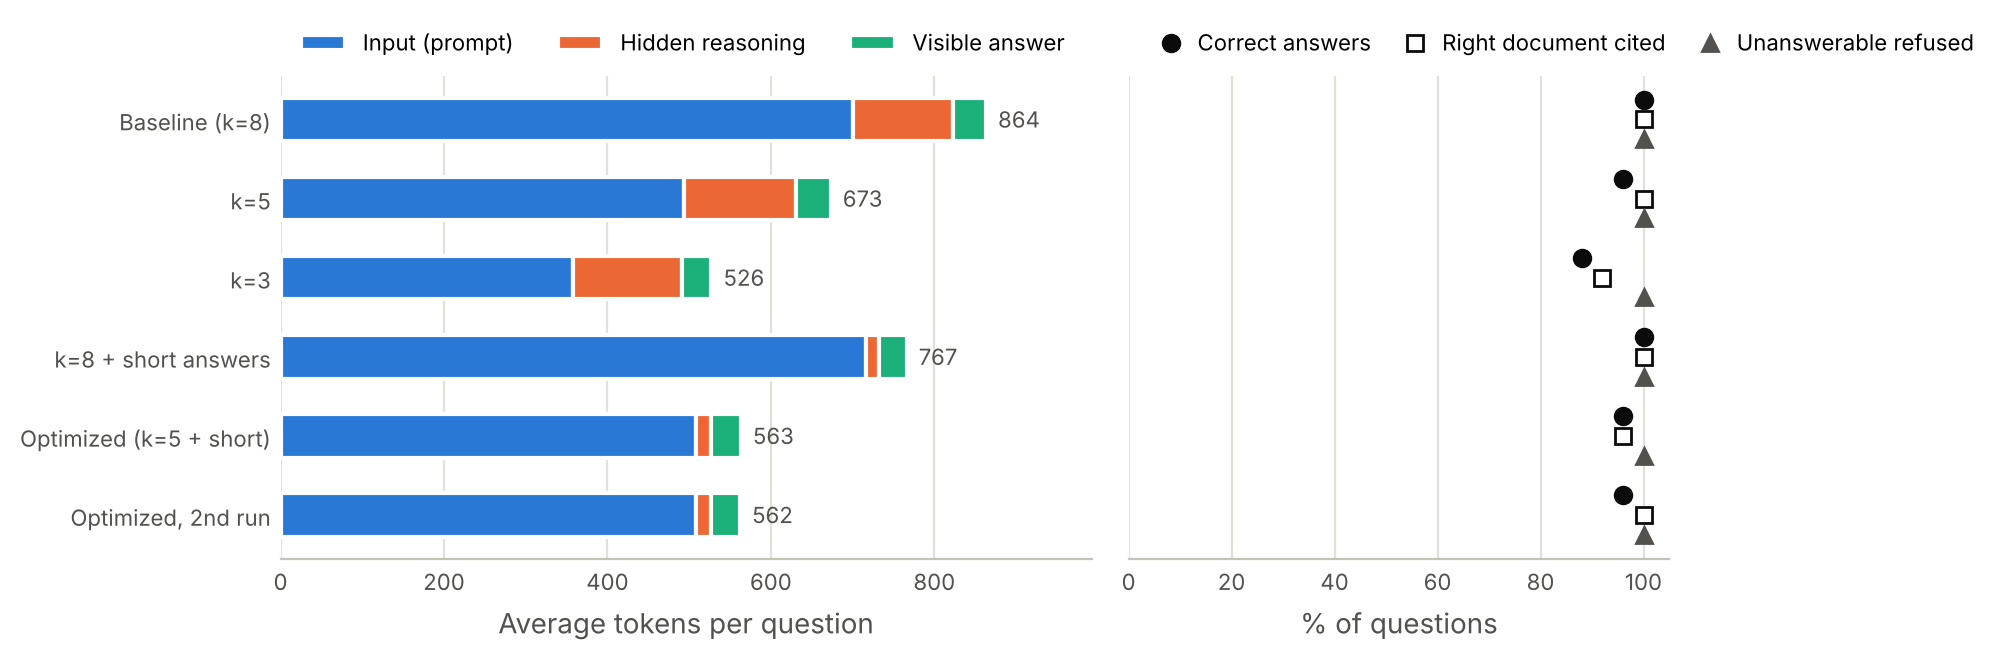
\includegraphics[width=\textwidth]{tokens_and_quality.png}
\caption{Token use (left) and answer quality (right) for each setting.}
\end{figure}

\vspace{-0.6em}
\textbf{What I learned.}
\begin{itemize}
\item \textbf{The optimized agent passed my quality rule.} It used 35\% fewer tokens per question (864 down to 563) and reduced the estimated cost by 46\%. It refused all 6 questions that the documents could not answer, and no answer was cut off. It missed only one question, q21. The earlier retrieval check had already predicted this: with $k{=}5$, the section containing the VPN server address was not retrieved, so the model returned the VPN profile instead.
\item \textbf{The biggest saving came from hidden reasoning.} I expected the three-sentence rule to make the visible answers much shorter, but gpt-oss-20b was already quite brief (40 to 34 visible tokens). Most of the saving came from reasoning, which dropped from 122 to 16 tokens per question. Groq's processing time was also cut by about half. Looking only at token totals would have been misleading: short answers alone saved 11\% of tokens but 32\% of the cost, while $k{=}5$ saved 22\% of tokens but only 10\% of the cost. This is because output tokens cost four times as much as input tokens.
\item \textbf{Reducing $k$ too much affected answer quality.} The free retrieval check was close to the results from the LLM: both expected and measured coverage were 100\% with $k{=}8$ and 96\% with $k{=}5$. With $k{=}3$, the check predicted 92\%, while the measured score was 88\%. The extra mistake with $k{=}3$ (q18) happened because the model left out ``every Friday'', not because search missed the information. For q14, where the required fact was missing, the model said it could not find the answer instead of making one up.
\item \textbf{A second run is useful.} The two optimized runs got the same correctness score and missed the same question. However, one citation changed (23 compared with 24). With a test this small, a difference of one question should therefore be interpreted carefully.
\end{itemize}

\textbf{Limits of this test.}
This was a small test with only 30 questions, so one question represents about 4 percentage points. The documents and questions were created with AI help and are cleaner than real company wiki pages. I tested only one model and only single questions, not long conversations. I checked answers by looking for keywords. I also reviewed the answers manually, but this method can still miss a correct answer that uses different wording. Finally, I selected $k$ using the same questions I later used for evaluation. A fairer test would use a separate set of questions.

\textbf{What I would try next.}
\begin{enumerate}
\item \textbf{Test long conversations.} This would let me evaluate chat-history summaries (idea~3).
\item \textbf{Improve search.} I would try embeddings and a reranker to see whether a smaller $k$ could still retrieve the right information.
\item \textbf{Add another evaluation method.} I would use an LLM-based evaluator, such as RAGAS~\cite{ragas}, alongside the keyword check.
\item \textbf{Test another model.} Different models use hidden reasoning in different ways, so the results may not be the same.
\end{enumerate}

\newpage
\section*{D. References}
\begingroup
\renewcommand{\section}[2]{}%
\small
\begin{thebibliography}{99}
\setlength{\itemsep}{0.15em}
\bibitem{lewis} P.~Lewis, E.~Perez, A.~Piktus et al. Retrieval-Augmented Generation for Knowledge-Intensive NLP Tasks. \emph{NeurIPS}, 2020. \url{https://arxiv.org/abs/2005.11401}
\bibitem{lostmiddle} N.~F.~Liu, K.~Lin, J.~Hewitt et al. Lost in the Middle: How Language Models Use Long Contexts. \emph{Transactions of the ACL}, 12, 2024. \url{https://arxiv.org/abs/2307.03172}
\bibitem{llmlingua} H.~Jiang, Q.~Wu, C.-Y.~Lin, Y.~Yang, L.~Qiu. LLMLingua: Compressing Prompts for Accelerated Inference of Large Language Models. \emph{EMNLP}, 2023. \url{https://arxiv.org/abs/2310.05736}
\bibitem{recomp} F.~Xu, W.~Shi, E.~Choi. RECOMP: Improving Retrieval-Augmented LMs with Compression and Selective Augmentation. \emph{ICLR}, 2024. \url{https://arxiv.org/abs/2310.04408}
\bibitem{memory} Q.~Wang, L.~Ding, Y.~Cao et al. Recursively Summarizing Enables Long-Term Dialogue Memory in Large Language Models. arXiv:2308.15022, 2023.
\bibitem{groqcache} Groq. Prompt caching (documentation). Accessed November 2026. \url{https://console.groq.com/docs/prompt-caching}
\bibitem{frugalgpt} L.~Chen, M.~Zaharia, J.~Zou. FrugalGPT: How to Use Large Language Models While Reducing Cost and Improving Performance. arXiv:2305.05176, 2023.
\bibitem{groqprice} Morph. Groq pricing (October 2026): GroqCloud API rates per model. \url{https://www.morphllm.com/groq-pricing}
\bibitem{groqreasoning} Groq. Reasoning (documentation). Accessed November 2026. \url{https://console.groq.com/docs/reasoning}
\bibitem{manning} C.~D.~Manning, P.~Raghavan, H.~Sch\"utze. \emph{Introduction to Information Retrieval}, chapter 6. Cambridge University Press, 2008.
\bibitem{gptoss} OpenAI. gpt-oss-120b \& gpt-oss-20b Model Card. arXiv:2508.10925, 2025.
\bibitem{groqlimits} Groq. Rate limits (documentation). Accessed November 2026. \url{https://console.groq.com/docs/rate-limits}
\bibitem{groqdeprecations} Groq. Model deprecations (documentation). Accessed November 2026. \url{https://console.groq.com/docs/deprecations}
\bibitem{ragas} S.~Es, J.~James, L.~Espinosa-Anke, S.~Schockaert. RAGAS: Automated Evaluation of Retrieval Augmented Generation. \emph{EACL (demos)}, 2024. \url{https://arxiv.org/abs/2309.15217}
\end{thebibliography}
\endgroup

\vspace{0.5em}
\textbf{How I used AI.}
I used Claude (Anthropic) as a helper during this exercise. I asked it about possible techniques and research papers, used it to prepare a first draft of the fictional documents and test questions, and got help with an early version of the code and with organising and wording this report. I ran the experiment myself using my own Groq API key. I also reviewed every answer whose score changed and went through the code until I could explain how each part worked.

\end{document}
